\section{Gold-PVD}
\label{goldpvd}

\todoline{Standardliteratur zitieren}

Als Testsystem für PVD-Prozesse bietet sich Gold-PVD an, mit der Goldschichten epitaktisch auf monokristallinen Substraten aufgewachsen werden können\cite{gottsche_uber_1956}, für amorphe oder polykristalline Substrate aber durch Bildung von Nanopartikeln polykristalline Schichten erzeugt werden\cite{svorcik_annealing_2011}.
Die Zielsetzung für die Untersuchungen der Gold-PVD bestehen in der Voruntersuchung des MD-Potentiales, der Simulation epitaktischer Abscheidungen auf dünnen und nanostrukturierten Gold-Substraten und der Simulation von Abscheidungen auf gröberen Strukturen.
Die genutzte EAM-Potentialparametrisierung wird mit dem LAMMPS-Paket\cite{plimpton_lammps_2014} verbreitet, basiert aber auf Parametern von \textsc{Foiles et al.}\cite{foiles_embedded-atom-method_1986}, die für die Einbettung einzelner Atome in Bulk- und Oberflächensysteme optimiert wurden und somit den Abscheidungsprozess auf atomistischer Ebene ideal darstellen sollten.

\subsection{Voruntersuchungen}

Zur Validierung grundlegender Materialeigenschaften von kristallinem Gold wurden Bindungslängen, Dichten und Koordinationszahlen aus einer relaxierten kristallinen Phase untersucht und mit experimentellen Werten\cite{haynes_crc_2011} verglichen (Tabelle~\ref{tab:goldpreresults}).
Eine gesammelte Übersicht der experimentellen Werte ist in Anhang~\ref{appendix_constants} zu finden.
In der MD-Simulation wurde ein Goldkristall mit einer Größe von \SI{40x40x40}{\angstrom} auf \SI{1000}{\kelvin} aufgeheizt (Schmelzpunkt: \SI{1337}{\kelvin}), im kanonischen Ensemble relaxiert und anschließend langsam abgekühlt, wobei die Dichte und die radiale Verteilungsfunktion bestimmt wurde.
Aus der radialen Verteilungsfunktion wurde anschließend die Bindungslänge und die Koordination bestimmt.

Bei diesem Prozess bleibt die Kristallstruktur erhalten und steht in guter Übereinstimmung mit den Literaturwerten.
Somit unterstützt die genutzte EAM-Para\-metri\-sierung das Zielsystem hinsichtlich der Dichte und Struktur monokristalliner Bulkmaterialien.

\begin{table}[hbt]
  \begin{threeparttable}
  \oddrowcolors
  \caption[Vergleich von strukturellen Eigenschaften von Gold]{
    Vergleich von strukturellen Eigenschaften von Gold mit experimentellen Daten als Voruntersuchung des PVD-Prozesses
  }
  \label{tab:goldpreresults}
  \begin{tabularx}{\textwidth}{|lXXXX|}
    \hline
    \textbf{unters. Größe} & \textbf{Temperatur} & \textbf{Simulation}                     & \textbf{Referenz}\tnote{a}              & \textbf{Abweichung} \\
    \hline
    Bindungslänge          & \SI{300}{\kelvin}   & \SI{2.885}{\angstrom}                   & \SI{2.884}{\angstrom}                   & \SI{0.05}{\percent} \\
    Koordination           & \SI{300}{\kelvin}   & \SI{12.00}{}                            & \SI{12.00}{}                            & \SI{0}{\percent}    \\
    Dichte                 & \SI{300}{\kelvin}   & \SI{18.99}{\gram\per\cubic\centi\meter} & \SI{19.30}{\gram\per\cubic\centi\meter} & \SI{-1.6}{\percent} \\
    Dichte                 & \SI{500}{\kelvin}   & \SI{18.89}{\gram\per\cubic\centi\meter} & \SI{19.13}{\gram\per\cubic\centi\meter} & \SI{-1.2}{\percent} \\
    \hline
  \end{tabularx}
  \begin{tablenotes}
    \item[a] Referenzwerte stammen aus dem \textit{CRC Handbook for Chemistry and Physics}\cite{haynes_crc_2011}
  \end{tablenotes}
  \end{threeparttable}
\end{table}

\subsection{Thermodynamische Eigenschaften}
\label{goldthermo}

Neben strukturellen Eigenschaften bilden EAM-Potentiale auch einige thermodynamische Eigenschaften von Metallen ab, die aufgrund der potentiell hohen Substrattemperaturen bei PVD-Prozessen\cite{gottsche_uber_1956} untersucht werden sollen.
Dafür wurde in MD-Simulationen ein \SI{40x40x40}{\angstrom} großer Block schrittweise von \SI{50}{\kelvin} auf \SI{2000}{\kelvin} erhitzt, wobei der Schmelzpunkt von \SI{1337}{\kelvin}\cite{haynes_crc_2011} überschritten wurde.
Die Relaxationszeit $t_\text{relax}$ für jeden Temperaturschritt und die Thermostat-Dämpfung $\tau$ wurden dabei variiert, um ihren Einfluss auf die Aussagekraft der Simulation zu untersuchen.
Die Ergebnisse (Abbildung~\ref{fig:goldthermo}) zeigen generell gute Übereinstimmung mit experimentellen Daten, wofür Relaxationszeiten $t_\text{relax} > \SI{20}{\pico\second}$ und Thermostat-Dämpfungsparameter $\tau \approx \SI{20}{\femto\second}$ bei einer Zeitschrittweite von $\Delta t = \SI{1}{\femto\second}$ für die Relaxation im isotherm-isobaren Ensemble als notwendig ermittelt wurden.
Bei geringeren $t_\text{relax}$ oder $\tau$ relaxiert das System innerhalb eines Temperaturschrittes nicht vollständig, wodurch der Schmelzpunkt überschätzt wird, wie in Abbildung~\ref{fig:goldthermo-b} zu sehen ist.
Darin zeigt sich auch eine Änderung in der Art des Phasenüberganges, der durch erhöhte Relaxationszeiten aufgrund von zeitlichen Effekten verzögert eintritt.
Das ergibt sich aus der Ähnlichkeit der Relaxationszeit zur Barostat-Dämpfung ($t_\text{relax}\approx \tau_p$), welche um Größenordnungen unter dem notwendigen Wert liegen (Abschnitt~\ref{mdmethods}), sodass sich das thermische Gleichgewicht nicht im Zeitrahmen der Simulation einstellen kann.

\begin{figure}[th]
  \captionsetup[subfigure]{singlelinecheck=false}
  \def\subfigwidth{7cm}
  \begin{subfigure}[t]{\subfigwidth}
    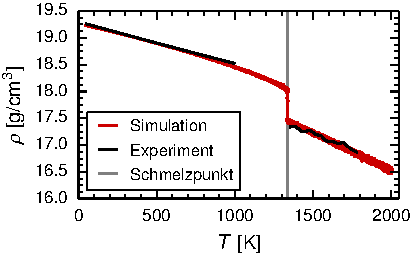
\includegraphics[width=\textwidth]{gold_bestthermo}
    \subcaption{Dichte bei $ t_\text{relax}=\SI{50}{\pico\second}$ und $\tau=\SI{0.02}{\femto\second}$}
    \label{fig:goldthermo-a}
  \end{subfigure}
  \hfill
  \begin{subfigure}[t]{\subfigwidth}
    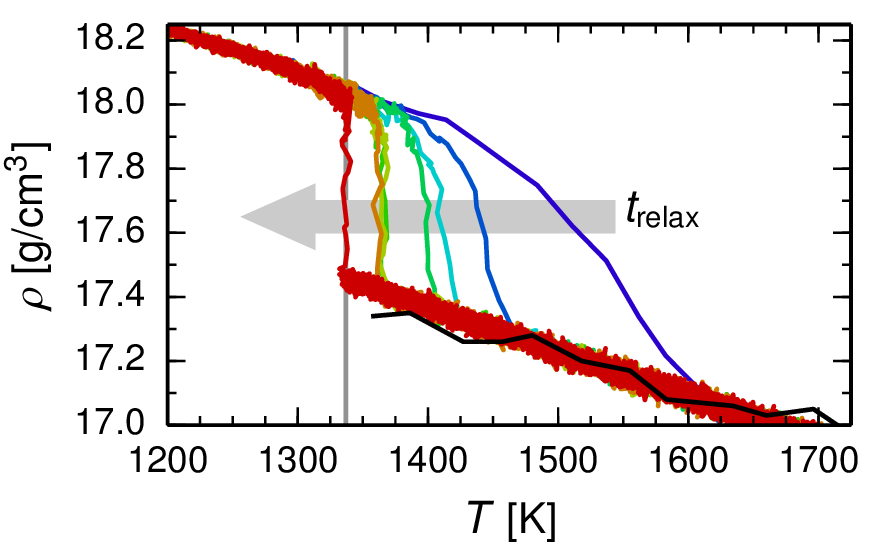
\includegraphics[width=\textwidth]{gold_relaxtime}
    \subcaption{Dichteänderung beim Schmelzen in Abh. der Relaxationszeit}
    \label{fig:goldthermo-b}
  \end{subfigure}
  \caption[Vergleich thermodynamischer Daten von Gold]{
    Vergleich thermodynamischer Daten von Gold.
    Experimentelle Werte stammen aus Standardliteratur sowie von \textsc{Brillo et al.}\cite{brillo_density_2006}.
  }
  \label{fig:goldthermo}
  \todoline{Legende der Relaxationszeiten fehlt}
\end{figure}

\subsection{Simulation des PVD-Prozesses}

In einer Parsivald-Simulation wurde auf einem kristallinen Substrat der Größe \SI{106x106}{\angstrom} \continuehere

Nach der Präparation eines Kristallsubstrates wurde es zusammen mit der EAM-Parametrisierung und weiteren Prozessparametern in einer Parsivald-Simulation eingelesen, wobei die Relaxationszeiten und Größen der MD-Simulationsräume aus den Vorbetrachtungen übernommen wurden.
Damit ergeben sich Reaktionsräume mit einer Größe von \SI{37x37x25}{\angstrom} mit jeweils ca. \num{1800} Atomen, Relaxationszeiten von \SI{1.4}{\nano\second} in \num{1400} Simulationsschritten und Auftreffgeschwindigkeiten von \SI{4}{\angstrom/\pico\second}.
Letztere liegen mit \SI{16.7}{\electronvolt} leicht oberhalb der üblichen Teilchenenergien von \SIrange{1}{10}{\electronvolt}\cite{thompson_ii._1968}, werden aber vor dem eigentlichen Auftreffen durch das Thermostat, welches unvermeidlich auch das auftreffende Atom betrifft, reduziert.
Zur Korrektur dieses systematischen Fehlers wäre eine Aufteilung des Integrators in einen kanonischen und einen mikrokanonischen Teil notwendig, was mit einem erhöhten Rechenaufwand für jede Simulation verbunden ist und deshalb bisher nicht umgesetzt wurde.

\todoline{Jörg: Verweis auf Vergleich mit Experimenten in 4.1.2 - ???}
Abbildungen~\ref{fig:golddepositions-a} und~\ref{fig:golddepositions-d} zeigen, wie eine Gold-Schicht auf dem kristallinen Substrat epitaktisch aufwächst.
Poren und Hohlräume wurden bei Untersuchungen der Alpha-Form~\ref{mdmethods-surface} nicht gefunden.
Abbildung~\ref{fig:goldroughness-a} stellt die Rauheit dar, die beim glatten Substrat über den Abscheidungszeitraum mit \SI{1.2}{\angstrom} konstant geblieben ist.
Fehler- und Abbruchraten bei den LAMMPS-Berechnungen lagen mit \SI{0.25}{\percent} unterhalb des aus den ALD-Prozessen der Bachelorarbeit erwarteten Wertes von \SI{5}{\percent}.

Mit einer Rauheit von \SI{1.2}{\angstrom} liegen die Werte um einen Faktor von \num{10} unterhalb der Literaturwerte\cite{svorcik_annealing_2011}, welche jedoch Gold-Sputtering auf einem Glas-Substraten untersucht haben.
Dadurch bilden sich polykristalline Schichten, bei denen die Bildung von Goldpartikeln den Wachstumsprozess dominiert, wo hingegen in den präsentierten Untersuchungen durch den Einfluss des monokristallinen Substrates und der gleichmäßig geringen Teilchenenergien epitaktisches Wachstum mit geringeren Rauheiten statt findet.
Obwohl Gold-Evaporation einen grundlegenden Prozess darstellt, konnten keine strukturellen Daten von Gold-PVD auf einem monokristallinen Substrat gefunden werden.
Aufgrund der hohen Mobilität der Gold-Atome auf der Oberfläche ergibt sich jedoch eine Affinität zu kristallinem Wachstum\cite{svorcik_annealing_2011,everitt_evolution_2000}, welche auch auf amorphen Substraten zu beobachten ist, auf monokristallinen Substraten jedoch zu epitaktischem Schichtwachstum führen sollte, wie es in den Parsivald-Simulationen beobachtet wurde.
Untersuchungen von Abscheidungssimulationen auf polykristallinen Gold-Substraten stehen noch aus, können aber helfen, den Einfluss der Partikelgröße von Gold auf polykristalline Substrate zu verstehen.

\subsubsection{Wachstum auf strukturierten Substraten}

Neben dem glatten Substrat wurden am Beispiel der Gold-PVD auch Abscheidungen auf strukturierten Substraten (Abbildung~\ref{fig:golddepositions}) mit identischen Prozessbedingungen simuliert.
Als Substrate wurden Stufen\todo{keine Stufe - was dann?} oder Spitzen mit einer Höhe von jeweils \SI{20}{\angstrom} und Neigungen von \SI{15}{\degree}, \SI{20}{\degree}, \SI{30}{\degree}, \SI{45}{\degree}, \SI{60}{\degree} und \SI{90}{\degree} präpariert.
Auf vorherige Relaxierung der Substrate wurde aufgrund der Prozessstabilität sowie der relaxierenden Eigenschaften der MD-Ereignisse verzichtet.
Zusätzlich wurden Lamellen und Säulen mit einer Strukturbreite von \SI{16}{\angstrom} (4 Kristall-Einheitszellen) zur Untersuchung eventueller Prozessartefakte präpariert, um Parsivald auf den Umgang mit nanoskopischen Störstellen zu untersuchen.
Diese Störstellen zeigten nach einer kurzen Relaxierung keine strukturellen Unterschiede zum glatten Substrat.

\begin{figure}
  \captionsetup[subfigure]{singlelinecheck=false}
  \def\subfigwidth{0.31\textwidth}
  \begin{subfigure}[t]{\subfigwidth}
    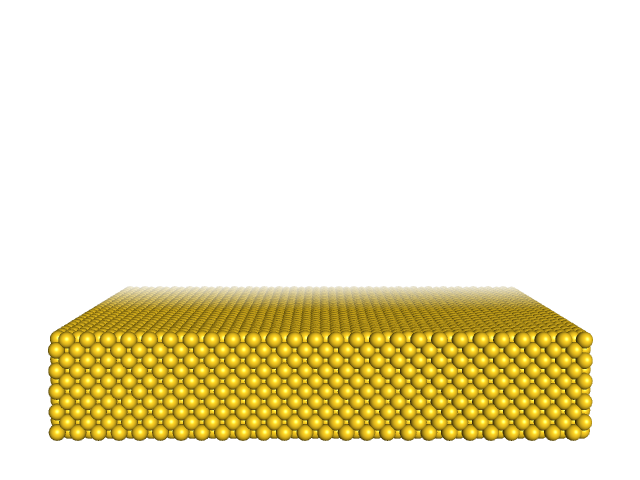
\includegraphics[width=\textwidth]{Au_substrate_flat}
    \subcaption{Glattes Gold-Substrat}
    \label{fig:golddepositions-a}
  \end{subfigure}
  \hfill
  \begin{subfigure}[t]{\subfigwidth}
    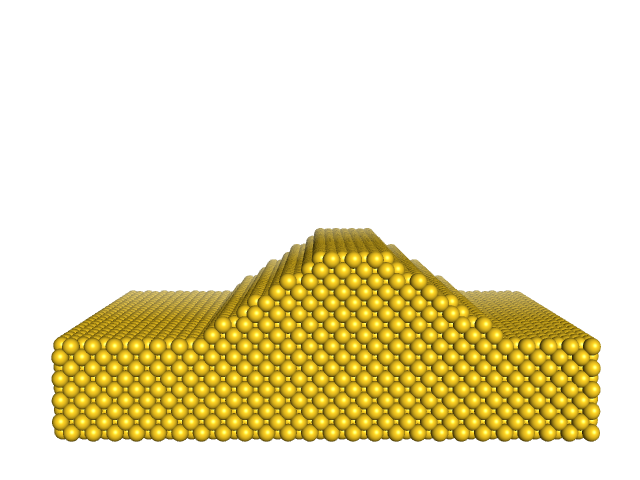
\includegraphics[width=\textwidth]{Au_substrate_step30}
    \subcaption{Gold-Stufe, \SI{30}{\degree}}
    \label{fig:golddepositions-b}
  \end{subfigure}
  \hfill
  \begin{subfigure}[t]{\subfigwidth}
    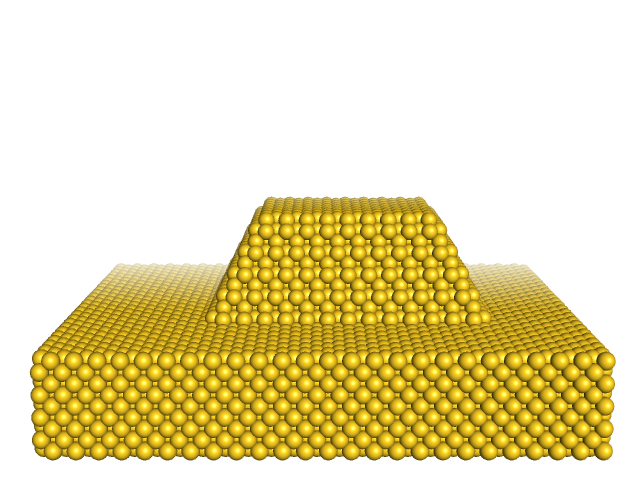
\includegraphics[width=\textwidth]{Au_substrate_tip60}
    \subcaption{Gold-Spitze, \SI{60}{\degree}}
    \label{fig:golddepositions-c}
  \end{subfigure}

  \LARGE\center{$\Downarrow$}
  \vspace{0.25cm}

  \captionsetup[subfigure]{singlelinecheck=false}
  \def\subfigwidth{0.31\textwidth}
  \begin{subfigure}[t]{\subfigwidth}
    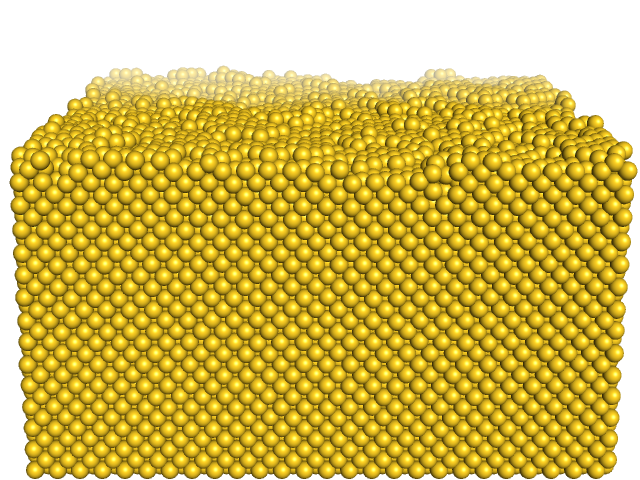
\includegraphics[width=\textwidth]{Au_deposition_flat}
    \subcaption{Glatte, kristalline Schicht ($\sigma_z = \SI{1.2}{\angstrom}$)}
    \label{fig:golddepositions-d}
  \end{subfigure}
  \hfill
  \begin{subfigure}[t]{\subfigwidth}
    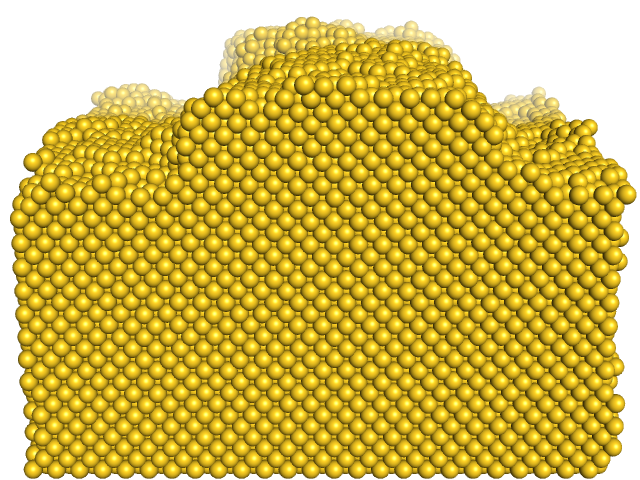
\includegraphics[width=\textwidth]{Au_deposition_step30}
    \subcaption{Fortsetzung der Stufe ($\sigma_z = \SI{6.4}{\angstrom}$)}
    \label{fig:golddepositions-e}
  \end{subfigure}
  \hfill
  \begin{subfigure}[t]{\subfigwidth}
    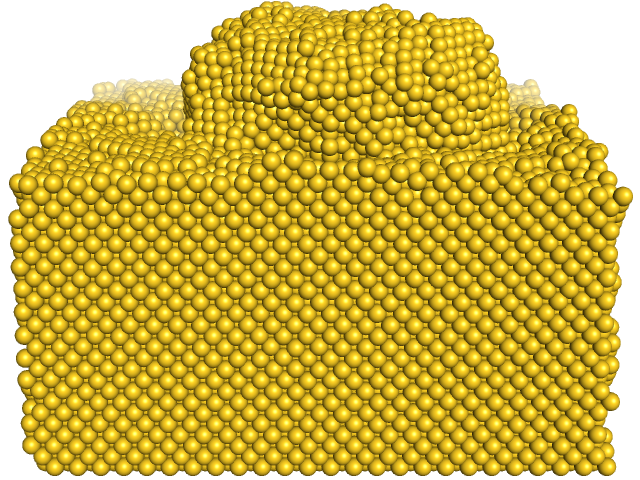
\includegraphics[width=\textwidth]{Au_deposition_tip60}
    \subcaption{Fortsetzung der Spitze ($\sigma_z = \SI{8.0}{\angstrom}$)}
    \label{fig:golddepositions-f}
  \end{subfigure}
  \caption[Gold-Abscheidung auf strukturierten Substraten]{
    Goldschicht nach 50 Abscheidungsschritten (\SI{47}{\angstrom}) auf strukturierten Substraten
  }
  \label{fig:golddepositions}
\end{figure}

\begin{figure}
  \captionsetup[subfigure]{singlelinecheck=false}
  \def\subfigwidth{0.49\textwidth}

  \begin{subfigure}[t]{\subfigwidth}
    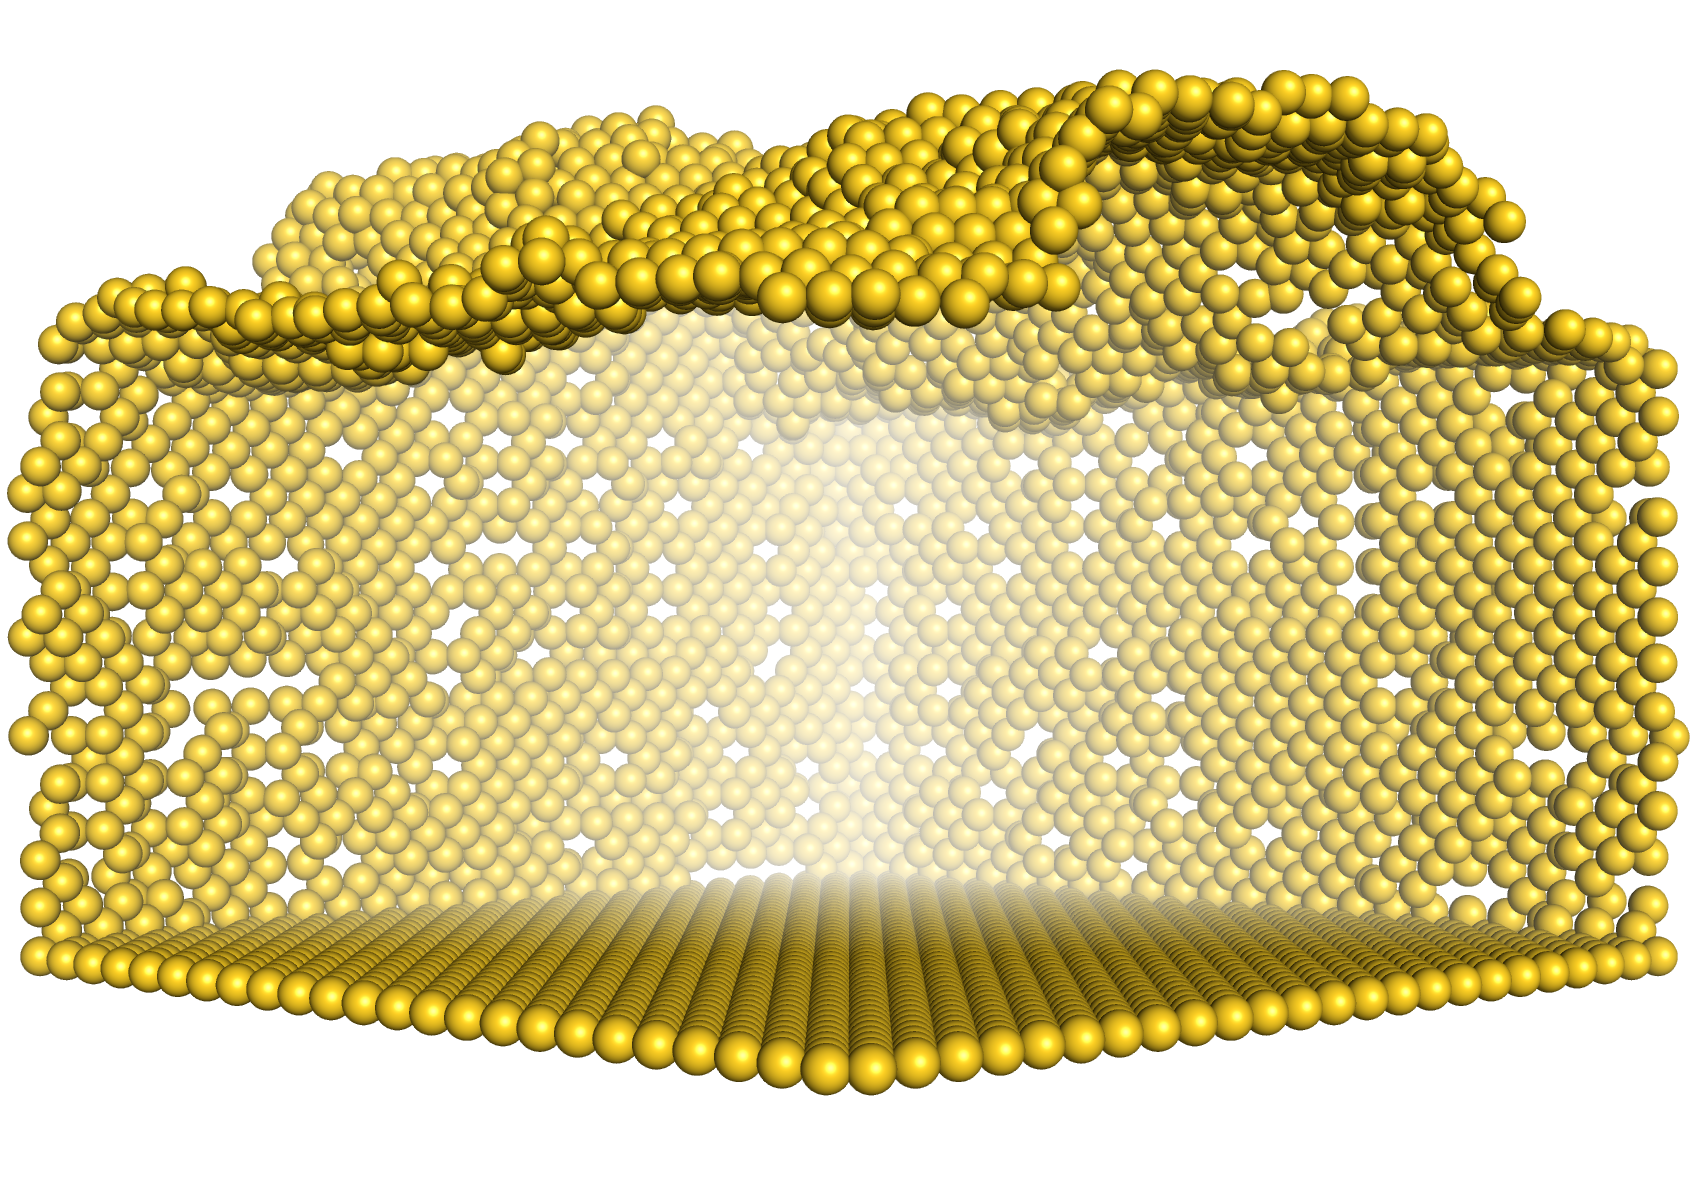
\includegraphics[width=\textwidth]{gold_step30_pockets}
    \subcaption{Alpha-Form der \SI{30}{\degree}-Stufe}
    \label{fig:goldpockets-a}
  \end{subfigure}
  \hfill
  \begin{subfigure}[t]{\subfigwidth}
    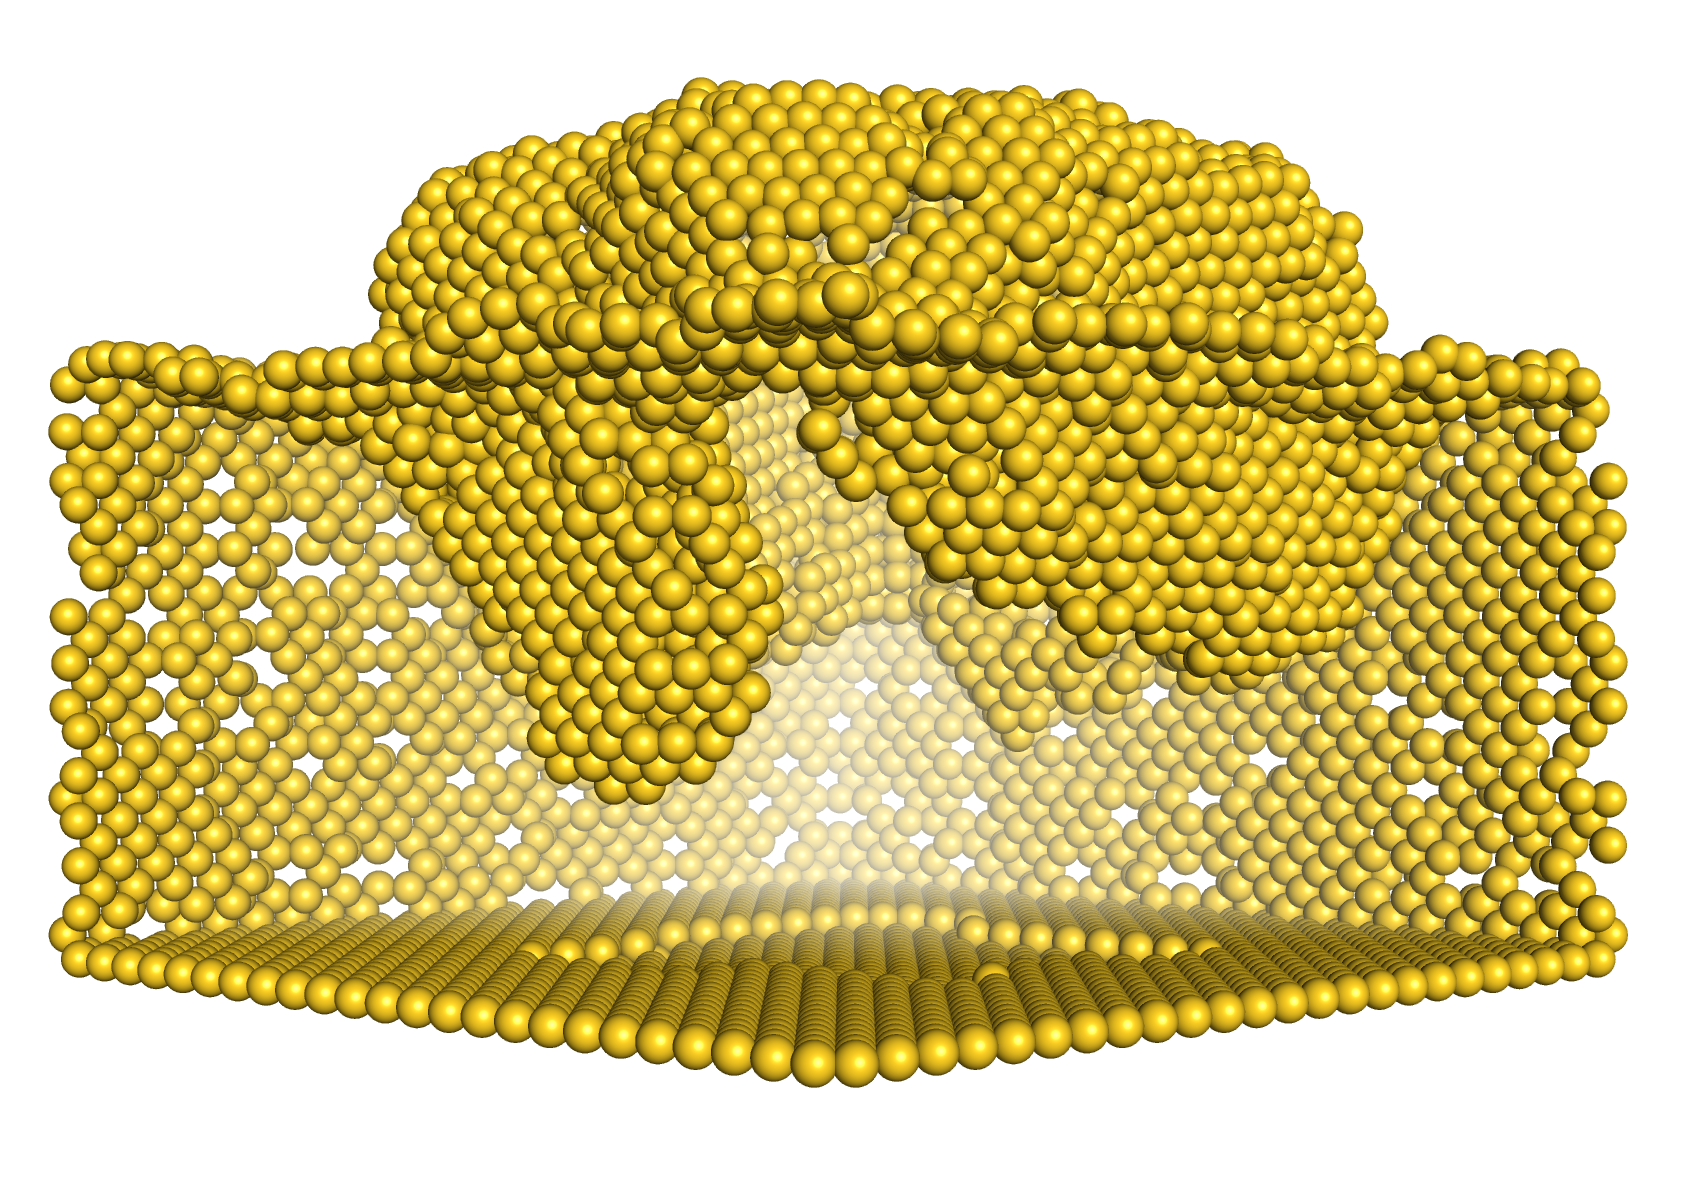
\includegraphics[width=\textwidth]{gold_tip90_pockets}
    \subcaption{Alpha-Form der \SI{90}{\degree}-Spitze}
    \label{fig:goldpockets-b}
  \end{subfigure}

  \caption[Porenbildung bei Gold-Strukturen]{Porenbildung bei Gold-Strukturen nach 40 Schritten (\num{22000} Ereignisse $\hat{=}$ \SI{38}{\angstrom}).
  }
  \label{fig:goldpockets}
\end{figure}

Wie die Alpha-Formen der simulierten Strukturen (Abbildung~\ref{fig:goldpockets-a}) zeigen, beinhaltet das abgeschiedene Gold bei geringen Neigungswinkeln keine Kristalldefekte, Poren oder Hohlräume.
Bei Abscheidungen auf Substrate hoher Neigungswinkel (>\SI{60}{\degree}) bilden sich Poren mit größerer Ausdehnung (>\SI{20}{\angstrom}).
Durch die Bildung von Überhängen an steilen Neigungen des Substrates werden die Poren zu Hohlräumen abgeschlossen, welche anschließend in der Schicht als Hohlräume verbleiben und somit ihre Dichte reduzieren und ihre Struktur stören.
Die Poren zeigen sich auch in den Oberflächenrauheiten der untersuchten Strukturen (Abbildung~\ref{fig:goldroughness}), bei denen für den extremen Fall der \SI{90}{\degree}-Steigung sogar lineare Zunahme gegen Ende der Simulation beobachtet werden kann.
Diese resultiert aus einem linearen Wachstum der Tiefe der Pore, die aus dem konstanten Wachstum der Schicht um sie herum resultiert.
Nach ihrem Abschluss zu einem Hohlraum sollte die Rauheit aber schlagartig abnehmen, wie im nachfolgenden Abschnitt~\ref{copperpvd} anhand von Kupfer beobachtet wurde.

\begin{figure}
  \captionsetup[subfigure]{singlelinecheck=false}
  \def\subfigwidth{0.49\textwidth}

  \begin{subfigure}[t]{\subfigwidth}
    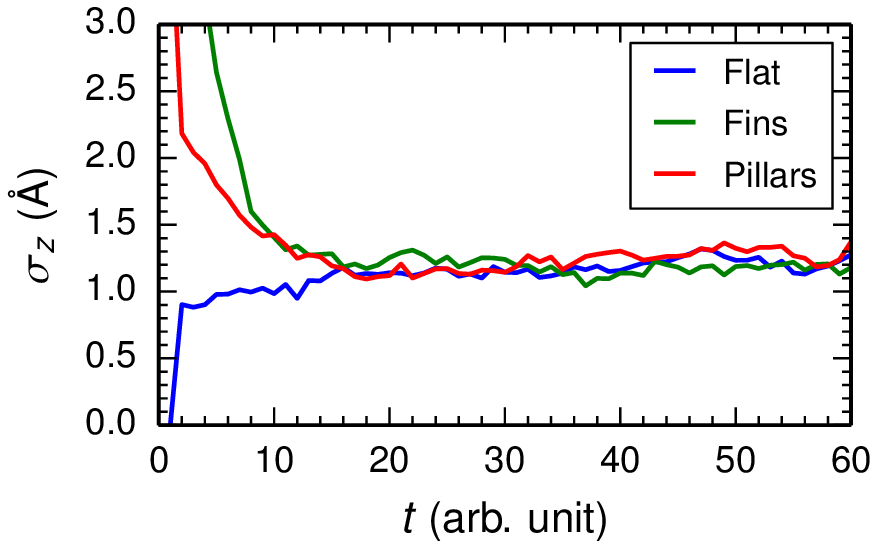
\includegraphics[width=\textwidth]{gold_goodroughness}
    \subcaption{RMS-Rauheit auf glatten Substraten}
    \label{fig:goldroughness-a}
  \end{subfigure}
  \hfill
  \begin{subfigure}[t]{\subfigwidth}
    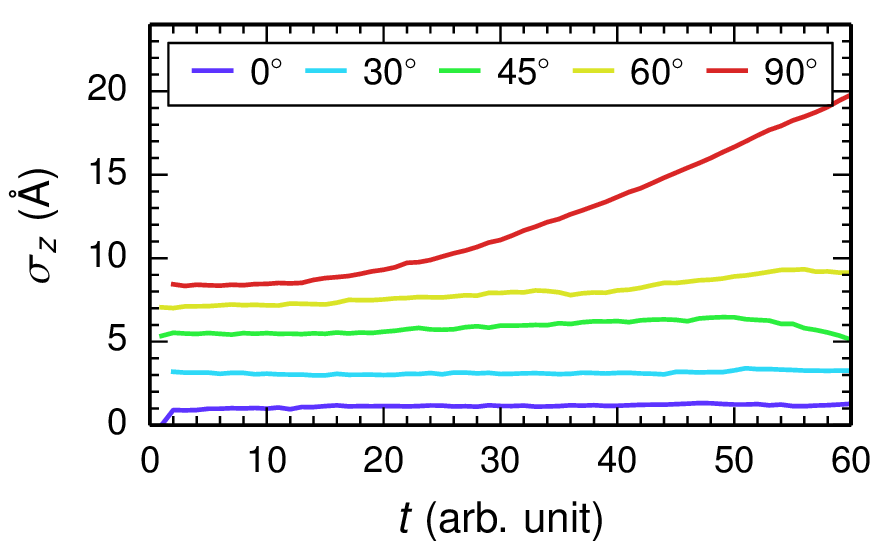
\includegraphics[width=\textwidth]{gold_tiproughness}
    \subcaption{Rauheit auf Spitzen von \SIrange{0}{90}{\degree}}
    \label{fig:goldroughness-b}
  \end{subfigure}

  \caption[Oberflächenrauheit von Gold]{
    Oberflächenrauheit von Gold auf verschiedenen Substraten (ideal: \SI{1.2}{\angstrom})
  }
  \label{fig:goldroughness}

\end{figure}

\begin{comment}
\subsection{Vergleich mit gesputterten Schichten}

Nachdem Gold in der Simulation erfolgreich aufgewachsen wurde, soll es nun auf Übereinstimmungen mit realen Schichten geprüft werden.
AFM-Untersuchungen gesputterter Goldschichten zeigen polykristallines Wachstum mit Rauheiten im Bereich von \SI{1.1}{\nano\meter} (etwa drei fcc-Kristallschichten)\cite{svorcik_annealing_2011}.
Dabei wird die Oberflächenrauheit von der Bildung von Nanopartikeln dominiert, deren Schmelztemperaturen mit der Größe der Partikel zunehmen\cite{liu_melting_2001}.
Kleinere Goldpartikeln verschmelzen oberhalb ihrer spezifischen Schmelztemperatur zu größeren Partikeln, wodurch die Rauheit der Goldoberfläche mit höheren Substrat- oder Annealing-Temperaturen steigt.
Bei Temperaturen unterhalb der Schmelztemperaturen, wie sie bei Sputtering vorhanden sind, werden durch Unterbindung der Verschmelzung kleiner Goldpartikel geringere Rauheiten erreicht, die mit längerer Sputterdauer weiter abnehmen\cite{svorcik_annealing_2011}.

In Parsivald-Simulationen ist dieser Trend bisher nur selten zu beobachten, wie etwa bei der \SI{45}{\degree}-Spitze, deren Rauheit gegen Ende der Simulation langsam abnimmt.
Die Ursachen liegen hier aber nicht in der Bildung und Verschmelzung von Nanopartikeln sondern der Schließung von Nanoporen, da die Schicht auch bei diesem Substrat per Epitaxie wächst.
Alle untersuchten Gold-Schichten wachsen epitaktisch senkrecht zur Kristallebene, jedoch zeigen Abscheidungssimulationen auf einigen strukturierten Substraten zusätzliche Porenbildung an Überhängen, die in der aktuellen Oberflächensuche begründet sind.
Für diese wird die Oberfläche und damit mögliche Ereignisorte parallel zur z-Achse gesucht, anstatt sie rechenaufwendig über die Alpha-Form aus einer Delaunay-Triangulation der Atompositionen zu bestimmen, wie es bereits zur Auswertung der simulierten Strukturen durchgeführt wird.
Somit werden höher gelegene Ereignisorte in der direkten Nachbarschaft bevorzugt, was sich in der Verstärkung von Überhängen bei strukturierten Substraten mit hohen Neigungswinkeln zeigt (Abbildung~\ref{fig:goldpockets-b}).
Als Lösung bieten sich die eben genannten Alpha-Formen (Abschnitt~\ref{datadelaunay}) an, deren Einbindung in das Parsivald-Programm noch aussteht.

Bei der Analyse der simulierten Strukturen wurde bei Abscheidungen auf glatten Substraten eine Rauheit von \SI{0.12}{\nano\meter} ermittelt, welche nur ca. \SI{10}{\percent} der experimentellen Werte beziehungsweise einer Lage von Goldatomen entspricht.
Strukturierte Substrate zeigen hier höhere Rauheiten, die zwar den experimentell bestimmten Rauheiten entsprechen (Abbildung~\ref{fig:goldroughness}), aber ebenfalls keine Nanopartikel enthalten, sondern aus epitaktisch gewachsenen, monokristallinen Schichten bestehen.
Daran lässt sich erkennen, dass die verwendeten MD-Simulations-Boxen zu klein und die Relaxationszeiten zu kurz sind, um die Bildung von Nanopartikeln darstellen zu können.
Zusätzlich verhindern kleine MD-Boxen in Verbindung mit monokristallinen Substraten die Ausbildung polykristalliner Strukturen, was sich im epitaktischen Wachstum monokristalliner Schichten äußert.
Derartige Finite-Size-Effekte sind Molekulardynamik-Simulationen inhärent, werden jedoch durch Parsivald für einige Systeme zusätzlich verstärkt.
Bei Abscheidung amorpher Schichten, wie für CVD- und ALD-Prozesse üblich, konnte dieser Effekt bisher nicht beobachtet werden (Abschnitt~\ref{siliconpvd}).
Eine Untersuchung einer Abscheidungssimulation auf polykristallinen Gold-Substraten steht noch aus.
\end{comment}

\clearpage
\subsection{Skalierbarkeit mit der Simulationsgröße}
\label{goldscalability}

Ein Vergleich mit den in Abschnitt~\ref{runtime} vorgestellten Laufzeitwerten wird im Folgenden anhand von Gold-PVD durchgeführt, für welche Abscheidungen auf unterschiedlich großen quadratischen Substraten mit Parsivald simuliert wurde.

Aus Messungen ergeben sich die elementaren Laufzeiten als $T_\text{E} = \SI{26}{\milli\second}$ und $T_\text{MD} = \SI{4.7}{\second}$, während $w_\text{MD} = \SI{37}{\angstrom}$ fest gewählt und $w_\text{sim}$ von \SI{106}{\angstrom} bis \SI{4}{\micro\meter} variiert wurde, wobei auch der für die Beschichtung von Nanoelektronik interessante Bereich von \SIrange{100}{1000}{\nano\meter} untersucht wurde.
Dabei wurde, durch verschiedene Störeinflüsse bedingt, eine unterschiedliche Anzahl an Parsivald-Zyklen durchlaufen, sodass die Laufzeiten keinen direkten Vergleich zulassen.

Die Ergebnisse der Untersuchungen sind in Tabelle~\ref{tab:goldscalability} zusammengefasst und stimmen gut mit den in Abschnitt~\ref{runtimeanalysis} ermittelten analytischen Werten überein (Abbildung~\ref{fig:goldscala}).
Die Zahl der möglichen Prozesse (Abbildung~\ref{goldscala-workers}) steht in guter Übereinstimmung mit $p_\text{max}$ für $\rho_\text{worker} = \SI{20}{\percent}$, wobei die maximale effiziente Substratbreite als $w_\text{eff} \approx \SI{100}{\nano\meter}$ ermittelt wurde.
Für die mit $p_\text{max}$ verwandten Workerdichten $\rho_\text{worker}$ ist eine leichte Abnahme von \SI{21.9}{\percent} für $w_\text{sim} = \SI{106}{\angstrom}$ zu \SI{10.3}{\percent} für $w_\text{sim} = \SI{1000}{\angstrom}$ erkennbar, die danach jedoch quadratisch mit der Substratbreite abnimmt.
Es existiert ein Ausreißer bei $w_\text{sim} = \SI{1}{\micro\meter}$, für den nur 46 Worker gestartet wurden ($\num{46} < p_\text{max} \approx \num{190}$), die zudem durch einen inzwischen behobenen Fehler im Host-Worker-Code auf einen Wert von \num{25.4} unterschätzt wurden.

Ein Vergleich der Laufzeiten mit Werten für $T_p$ aus Gleichung~\ref{eq:runtime} zeigt ebenfalls gute Übereinstimmungen, wobei der Ausreißer bei $w_\text{sim} = \SI{1}{\micro\meter}$ ebenfalls erkennbar ist.
Aufgrund des Wachstums von Schichten unterschiedlicher Dicke ist ein direkter Vergleich nicht aussagekräftig, doch bestätigt die Übereinstimmung mit den analytischen Werten die gute Skalierbarkeit von Parsivald mit der Substratbreite.

\begin{table}[H]
  \begin{threeparttable}

    \caption{Untersuchungen zur Skalierbarkeit von Parsivald}
    \label{tab:goldscalability}

    \begin{tabularx}{\textwidth}{|Xrrrrrrr|}
      \hline
      \textbf{$w_\text{sim}$} & \textbf{Wachst.}    & \textbf{Atome} & \textbf{$N_\text{E}$} & \textbf{Worker\tnote{a} $p$}          & \textbf{$\rho_\text{work.}$} & \textbf{$T_\text{p}$} & \textbf{RAM}\tnote{b} \\
      \hline
      \SI{106}{\angstrom}     & \SI{70}{\angstrom}  & \num{59549}    & \num{46030}           & \num{1.8}\tnote{c}        (\num{4})   & \SI{21.9}{\percent}          & \SI{32.2}{\hour}      & \SI{254}{\mebi\byte}  \\
%%    \SI{204}{\angstrom}     & \SI{42}{\angstrom}  & \num{152374}   & \num{102374}          & \num{14.5}\tnote{c}       (\num{18})  & \SI{13.9}{\percent}          & \SI{25.5}{\hour}      & \SI{257}{\mebi\byte}  \\
      \SI{204}{\angstrom}     & \SI{38}{\angstrom}  & \num{142835}   & \num{92835}           & \num{5.32}\tnote{c}       (\num{12})  & \SI{17.5}{\percent}          & \SI{22.1}{\hour}      & \SI{257}{\mebi\byte}  \\
      \SI{500}{\angstrom}     & \SI{93}{\angstrom}  & \num{1708600}  & \num{1401081}         & \num{24.8}\tnote{c}       (\num{50})  & \SI{13.6}{\percent}          & \SI{73.6}{\hour}      & \SI{397}{\mebi\byte}  \\ % \SI{282}{\mebi\byte}
%%      \SI{1000}{\angstrom}  & \SI{5.4}{\angstrom} & \num{1591908}  & \num{381588}          & \num{44.8}                (\num{46})  & \SI{6.1}{\percent}           & \SI{1.5}{\hour}       & \SI{368}{\mebi\byte}  \\
      \SI{1000}{\angstrom}    & \SI{92}{\angstrom}  & \num{6733948}  & \num{5539942}         & \num{75.4}\tnote{c}       (\num{149}) & \SI{10.3}{\percent}          & \SI{97.5}{\hour}      & ~                     \\
      \SI{1}{\micro\meter}    & \SI{1.3}{\angstrom} & \num{1.3e8}    & \num{8186990}         & \num{25.4}\tnote{d}       (\num{46})  & \SI{0.03}{\percent}          & \SI{117.5}{\hour}     & \SI{11.5}{\gibi\byte} \\
%%    \SI{2}{\micro\meter}    & \SI{0.4}{\angstrom} & \num{4.9e8}    & \num{10356031}        & \num{26.3}\tnote{d}       (\num{46})  & \SI{0.009}{\percent}         & \SI{117.5}{\hour}     & ~                     \\
      \SI{2}{\micro\meter}    & \SI{1.0}{\angstrom} & \num{5.1e8}    & \num{25855695}        & \num{189}\tnote{e}        (\num{245}) & \SI{0.06}{\percent}          & \SI{186.8}{\hour}     & \SI{45.4}{\gibi\byte} \\
      \SI{4}{\micro\meter}    & ~                   & \num{1.9e9}    & ~                     & ~                         ~           & ~                            & ~                     & \SI{182}{\gibi\byte}  \\
      \hline
    \end{tabularx}

    \begin{tablenotes}
    \item[a] Mittelwert $p$ und beobachtetes Maximum der Zahl paralleler Worker
    \item[b] Vom Hostprozess verbrauchter Arbeitsspeicher.
    \item[c] $p = p_\text{max,1}$: Maximale Workerdichte erreicht
    \item[d] Inzwischen behobener Fehler in Parsivald hat Workerneustart verhindert
    \item[e] $p = p_\text{max,2}$: Ereignis-Durchsatz des Hostprozesses erreicht
    \end{tablenotes}

  \end{threeparttable}
\end{table}

Zuletzt zeigt die Auswertung der vom Hostprozess verbrauchten Ressourcen  einen Speicherverbrauch von $\text{RAM} = \SI{253}{\mebi\byte} + \SI{94}{\byte} \cdot N_\text{Atome}$, womit auch große Simulationen mit \num{1.9e9} Atomen mit nur \SI{186}{\gibi\byte} Arbeitsspeicher durchgeführt werden können (Abbildung~\ref{fig:goldscala-b}).
Somit stellt der verfügbare Arbeitsspeicher aktuell nur ein untergeordnetes Kriterium dar, jedoch spiegelt sich diese Größe auch in den atomistischen Dateien wider, die von Parsivald erzeugt werden, und somit nicht mehr effizient ausgewertet werden können, weshalb eine Auswertung zur Ausführungszeit notwendig wäre.

Somit bestätigen sich einige Vorhersagen aus Abschnitt~\ref{runtime}, jedoch sind weitere Untersuchungen, etwa hinsichtlich der Ereignis-Laufzeit $T_\text{E}$, für einen umfassenden Vergleich notwendig.

\vspace{2em}

\begin{figure}[H]
  \centering
  \captionsetup[subfigure]{singlelinecheck=false}
  \def\subfigwidth{7cm}
  \begin{subfigure}[t]{\subfigwidth}
    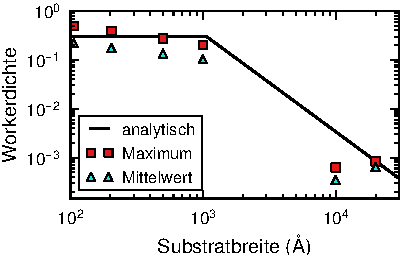
\includegraphics[width=\textwidth]{workerdichte}
    \subcaption{Workerdichte auf der Oberfläche (1=ideal)}
    \label{fig:goldscala-density}
  \end{subfigure}
  \hfill
  \begin{subfigure}[t]{\subfigwidth}
    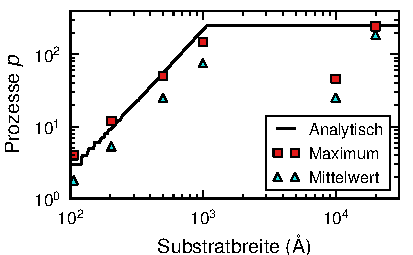
\includegraphics[width=\textwidth]{workers}
    \subcaption{Parallele Prozesse}
    \label{fig:goldscala-workers}
  \end{subfigure}

  \vspace{1em}

  \begin{subfigure}[t]{\subfigwidth}
    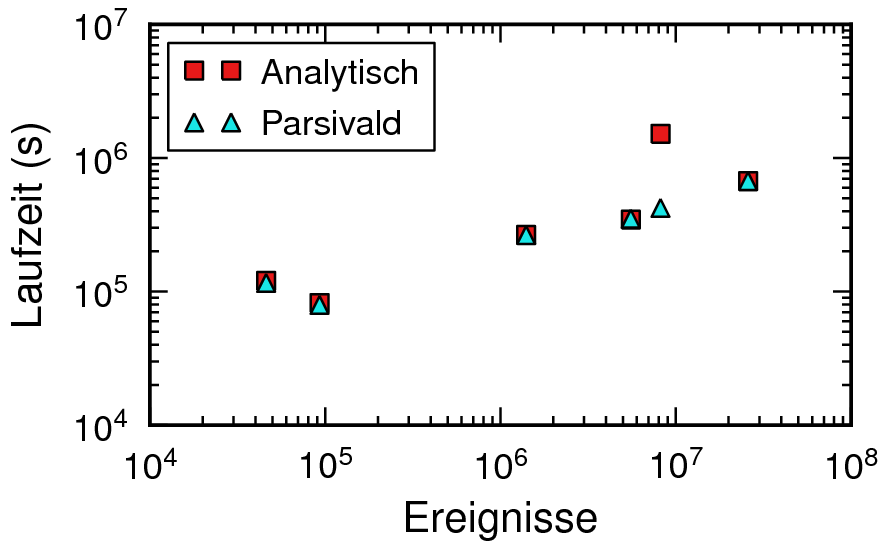
\includegraphics[width=\textwidth]{runtime}
    \subcaption{Laufzeit verschiedener Simulationen}
    \label{fig:goldscala-runtime}
  \end{subfigure}
  \hfill
  \begin{subfigure}[t]{\subfigwidth}
    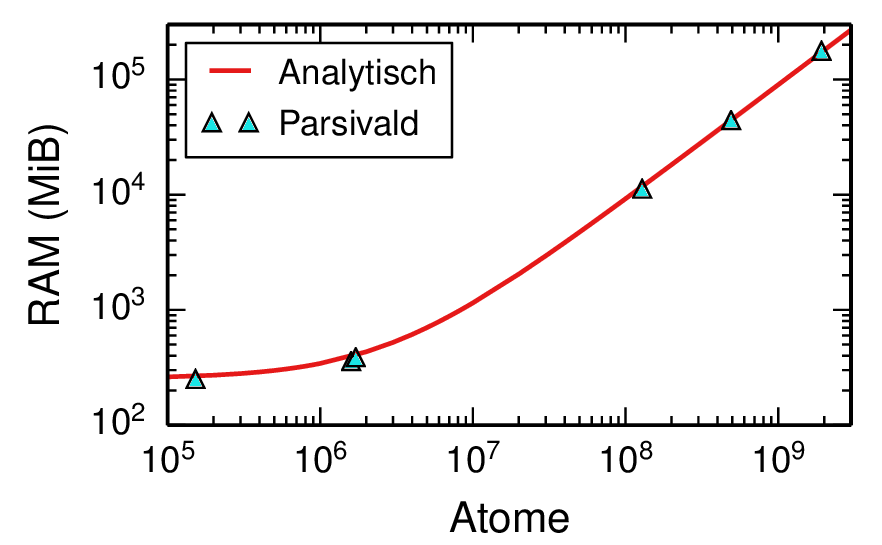
\includegraphics[width=\textwidth]{memory}
    \subcaption{Speicherverbrauch der Simulation}
    \label{fig:goldscala-memory}
  \end{subfigure}
  \caption{Parallelisierungseigenschaften von Parsivald}
  \label{fig:goldscala}
\end{figure}
